\documentclass{article}

\usepackage{titlesec}
\titlelabel{\thetitle.\quad}
\usepackage{amsmath}
\usepackage{amssymb}
\usepackage{mathtools}
\usepackage{enumitem}
\usepackage{tkz-graph}
\usetikzlibrary{positioning}

\setlength{\textwidth}{7in}
\setlength{\evensidemargin}{-0.24in}
\setlength{\oddsidemargin}{-0.24in}
\setlength{\textheight}{8.45in}
\setlength{\topmargin}{-0.45in}
\setlength{\parindent}{0.3in}
\headheight20pt
\headsep22pt

\pagestyle{myheadings}
\usepackage{fancyhdr}
\renewcommand{\headrulewidth}{0pt}
\usepackage{mathtools}
\usepackage{amsmath}

\pagestyle{fancy}
\fancyhf{}
\pagenumbering{arabic}
\lhead{\large\textbf{ Jason Li - 101310366} \hfill \thepage \vspace{-5pt}\\\hrulefill}


\begin{document}
\bibliographystyle{alpha}
\title{Assignment 1 - COMP 2804}
%\date{} %Uncomment this if you do not want the date to be shown.
\maketitle
\thispagestyle{fancy}
\noindent
\pagenumbering{arabic}

\medskip

\section{Extension of the Erdős–Rényi–Sós Friendship Theorem}

Given that we know that a complete graph $K_6$ has at least one monochromatic cycle:

\begin{enumerate}
    \item We know that a complete graph $K_6$ whose edges consist of 2 colors has at least one monochromatic cycle. Within that cycle, each of its vertices has at least 2 edges that are one color which forms the cycle, and 3 others of any color. Based on this, we can conclude the following: 
\begin{itemize}
    \item If any of the remaining 3 edges connected to any of the vertices in the monochromatic cycle were the same color as the cycle itself, this would produce a monochromatic lollipop. 

    \begin{center}
        \begin{tikzpicture}[scale=0.70, every node/.style={scale=0.9}]
        \node[draw, circle] (a1) at (150:3) {a1};
        \node[draw, circle] (a2) at (210:3) {a2};
        \node[draw, circle] (a3) at (270:3) {a3};
        \node[draw, circle] (b1) at (90:3) {b1};
        \node[draw, circle] (b2) at (30:3) {b2};
        \node[draw, circle] (b3) at (330:3) {b3};

        \draw[blue, line width=1mm] (a1) -- (a2);
        \draw[blue, line width=1mm] (a2) -- (a3);
        \draw[blue, line width=1mm] (a1) -- (a3);
        \draw[blue!15, line width=1mm] (a1) -- (b1);
        \draw[blue!15, line width=1mm] (a1) -- (b2);
        \draw[blue!15, line width=1mm] (a1) -- (b3);
        \end{tikzpicture}
        \\ \vspace{5mm}\
        Any connection to the cycle via $a_1$ creates a lollipop. We can observe that the same is true for $a_2$ and $a_3$.
    \end{center}
    
    \item Assume the monochromatic cycle is blue. If all of the 3 vertices in the monochromatic cycle had their remaining 3 edges be red, then in the cycle $a_1, a_2, a_3$, each vertex has a red edge connecting it to $b_1, b_2$ and $b_3$. We thus have red edges $a_ib_j$ for each $i,j \in \{1, 2, 3\}$ which fulfills the definition of a $K_{3,3}$ graph.
    \begin{center}
        \begin{tikzpicture}[scale=0.70, every node/.style={scale=0.9}]
        \node[draw, circle] (a1) at (150:3) {a1};
        \node[draw, circle] (a2) at (210:3) {a2};
        \node[draw, circle] (a3) at (270:3) {a3};
        \node[draw, circle] (b1) at (90:3) {b1};
        \node[draw, circle] (b2) at (30:3) {b2};
        \node[draw, circle] (b3) at (330:3) {b3};

        \draw[blue, line width=1mm] (a1) -- (a2);
        \draw[blue, line width=1mm] (a2) -- (a3);
        \draw[blue, line width=1mm] (a1) -- (a3);
        \draw[red, line width=1mm] (a1) -- (b1);
        \draw[red, line width=1mm] (a1) -- (b2);
        \draw[red, line width=1mm] (a1) -- (b3);
        \draw[red, line width=1mm] (a2) -- (b1);
        \draw[red, line width=1mm] (a2) -- (b2);
        \draw[red, line width=1mm] (a2) -- (b3);
        \draw[red, line width=1mm] (a3) -- (b1);
        \draw[red, line width=1mm] (a3) -- (b2);
        \draw[red, line width=1mm] (a3) -- (b3);
        \end{tikzpicture}
        Red $K_{3,3}$
    \end{center}
\end{itemize}
\end{enumerate}

Thus we have proven that any complete graph $K_6$ colored with 2 colors, must contain either a monochromatic lollipop or monochromatic $K_{3,3}$. If we choose to make the monochromatic triangle red instead, the same result will occur with the colors inverted.

\section{Proving a binomial identity}
    To create a bijective function $f : S_0 \rightarrow S_1$, we need to make a function that for every element of $S_0$, there will be a single unique element $S_1$. Consider the following function

    \begin{tabular}{c|l}
         & Take a random element x where $x \in S$ \\
         & Let $\{e_1, ... ,e_n\}$ be the elements of $S_0$ and $\{o_1, ... , o_m\}$ be the elements of $S_1$ \\
         & For i in n: \\
         & \hspace{5mm} If $x \in e_i$, remove x from $e_i$ \\
         & \hspace{5mm} If $x \not\in e_i$, add x to $e_i$ \\
    \end{tabular}
    
    If we take a set with an even number of elements and either add or remove one, we will always end up with a set of odd numbers. Since all elements in the subsets including x are in $S$, for each set in $S_0$ there will be a a set in $S_1$ that is mapped onto by the function. Note that if $e_i = S$, $x \in e_i$ so we will never get a set that is greater than $S$.

\section{A summation game}
Let's play a game. We start with a list of numbers $1, 2, 3, \dots, 2024$. We take turns by picking two numbers from the list, say $a$ and $b$, and removing them. Then, we insert exactly one of the numbers $|a-b|$ or $a+b$ into the list. Note that the length of the list decreases by one after each change. The game stops when only one number is left on the list. Prove that the final remaining number is even. \\
The summation of the sequence is:
\begin{eqnarray*}
    \sum_{i=1}^{2024} i & = & \frac{2024(2025)}{2} \\
    & = & 2049300
\end{eqnarray*}
$\therefore$ The summation of the sequence is an even number. \\
When we remove 2 numbers $a$ and $b$, and insert a + b, the sum remains the same since $\sum 0 = 0$ \\
When we remove 2 numbers $a$ and $b$, and insert $|a-b|$, the sum is reduced by either $2a$ or $2b$, depending on which is lesser. In this case, the sum will always remain even because $\sum 2n$ = $2\sum n$ where is is some integer. \\
$\therefore$ Every time we change the list, the sum remains even.\\
$\therefore$ When there is only one number left, that number must be even for the sum of the list to be even. $\square$

\section{A predicate logic exercise}
Prove that Resolution is valid using the laws of propositional logic and any of the other rules of inference besides Resolution. \\
To get to $b \lor c$ given the following arguments: \\
\begin{enumerate}[label =(\arabic*), ref = \arabic*]
\item $a \lor b$ 
\item $\neg a \lor c$ 
\vspace{5pt} \hrule \vspace{5pt}
\item $(a \implies c)$ \hfill Implication Relation (2) 
\item $(\neg a \implies b)$ \hfill Implication Relation (1) 
\item $(\neg b \implies \neg \neg a)$ \hfill Contrapositive (4) 
\item $(\neg b \implies a)$ \hfill Double Negation (5) 
\item $\neg b \implies c$ \hfill Hypothetical Syllogism (6, 3) 
\item $b \lor c$ \hfill Implication Relation (6) 
\end{enumerate}
\hfill $\square$

\section{Proof by induction}
To prove the closed form for the following recursive function: $$ f(n) = 
    \begin{cases}
    0 \hspace{100px} \text{ where } n = 0 \\
    1 \hspace{100px} \text{ where } n = 1 \\
    4 \cdot f(n-2) \hspace{55px} \text{ where } n \geq 2
    \end{cases} 
    $$
Base Cases: $f(0) = 2^{k-2}((-1)^{k+1}+1) = 0$, $f(1) = 2^{k-2}((-1)^{k+1}+1) = 1$ \\
    Inductive Hypothesis: $f(k) = 2^{k-2}((-1)^{k+1}+1)$ for all $k \in \{0,...,n-1\}$
    \begin{equation}
        \begin{split}
            f(n) &= 4 \times f(n-2)\\
            &= 4 \times (2^{k-4}((-1)^{k-1}+1) \\
            &= 2^{k-2}((-1)^{k-1}+1 \\
            &= 2^{k-2}(\frac{-1 \times -1}{-1 \times -1}(-1)^{k-1}+1) \\
            &= 2^{k-2}\frac{(-1)^2(-1)^{k-1}+1}{1}\\
            &= 2^{k-2}((-1)^{k+1}+1)
        \end{split}
    \end{equation}
    This is equal to the inductive hypothesis so we have proven that it is equal to the recursive function.
    
\end{document}
